%% ============================================================
%%  MLOps Report — Bug Hunter RL
%%  Course: Machine Learning Operations (24AM6AEMLO)
%%  B.M.S College of Engineering, VTU
%% ============================================================
\documentclass[12pt,a4paper]{report}

%% ---- Packages -----------------------------------------------
\usepackage[a4paper, left=1in, right=1in, top=0.88in, bottom=0.75in]{geometry}
\usepackage{mathptmx}          % Times New Roman
\usepackage[T1]{fontenc}
\usepackage[utf8]{inputenc}
\usepackage{setspace}
\usepackage{graphicx}
\usepackage{float}
\usepackage{caption}
\usepackage{subcaption}
\usepackage{booktabs}
\usepackage{tabularx}
\usepackage{longtable}
\usepackage{array}
\usepackage{multirow}
\usepackage{amsmath}
\usepackage{amssymb}
\usepackage{listings}
\usepackage{xcolor}
\usepackage{enumitem}
\usepackage{fancyhdr}
\usepackage{titlesec}
\usepackage{tocloft}
\usepackage{emptypage}
\usepackage{url}
\usepackage[hidelinks]{hyperref}

%% ---- Page style ---------------------------------------------
\pagestyle{fancy}
\fancyhf{}
\fancyhead[L]{\small\textit{Autonomous Software Bug Hunter using Reinforcement Learning}}
\fancyhead[R]{\small\textit{BMSCE, Dept. of ML}}
\fancyfoot[C]{\thepage}
\renewcommand{\headrulewidth}{0.4pt}

\fancypagestyle{plain}{
  \fancyhf{}
  \fancyfoot[C]{\thepage}
  \renewcommand{\headrulewidth}{0pt}
}

%% ---- Chapter/Section titles ---------------------------------
\titleformat{\chapter}[block]
  {\normalfont\fontsize{14}{17}\bfseries\centering}
  {CHAPTER \thechapter}{1em}{\MakeUppercase}
\titlespacing*{\chapter}{0pt}{10pt}{20pt}

\titleformat{\section}
  {\normalfont\fontsize{13}{16}\bfseries}
  {\thesection}{1em}{}
\titleformat{\subsection}
  {\normalfont\fontsize{12}{15}\bfseries}
  {\thesubsection}{1em}{}

%% ---- ToC formatting -----------------------------------------
\renewcommand{\cftchapfont}{\bfseries}
\renewcommand{\cftsecfont}{}
\renewcommand{\cftchapleader}{\cftdotfill{\cftdotsep}}
\setlength{\cftbeforechapskip}{6pt}

%% ---- Listings (code) ----------------------------------------
%% YAML language definition for listings
\lstdefinelanguage{yaml}{
  keywords={true, false, null, yes, no},
  sensitive=false,
  comment=[l]{\#},
  morestring=[b]',
  morestring=[b]",
}

\lstset{
  basicstyle=\ttfamily\small,
  keywordstyle=\bfseries\color{blue!70!black},
  commentstyle=\itshape\color{green!50!black},
  stringstyle=\color{orange!80!black},
  breaklines=true,
  frame=single,
  numbers=left,
  numberstyle=\tiny\color{gray},
  numbersep=6pt,
  showstringspaces=false,
  captionpos=b,
}

%% ---- Paragraph spacing --------------------------------------
\setlength{\parindent}{0pt}
\setlength{\parskip}{6pt}
\onehalfspacing

%% ---- Custom commands ----------------------------------------
\newcommand{\sectionline}{\noindent\rule{\linewidth}{0.4pt}}
\newcommand{\btitle}{Autonomous Software Bug Hunter using Reinforcement Learning}
\newcommand{\coursename}{Machine Learning Operations}
\newcommand{\coursecode}{24AM6AEMLO}
\newcommand{\deptname}{Machine Learning}
\newcommand{\collegename}{B.M.S COLLEGE OF ENGINEERING}
\newcommand{\uniline}{(An Autonomous Institute, Affiliated to VTU)}
\newcommand{\collegeaddr}{P.O. Box No.~1908, Bull Temple Road, Bengaluru -- 560\,019}
\newcommand{\ay}{A.Y 2025--26}
\newcommand{\hodname}{Dr.~M Dakshayini}
\newcommand{\principalname}{Dr.~Bheemsha Arya}

%% ---- Student info (fill in USNs) ----------------------------
\newcommand{\studentA}{Akshat Baranwal \quad (USN:~1BM22AI009)}
\newcommand{\studentB}{Rahul H          \quad (USN:~1BM22AI\textit{[FILL]}\,)}
\newcommand{\studentC}{\textit{[Student 3 Name]}  \quad (USN:~1BM22AI\textit{[FILL]}\,)}
\newcommand{\semSection}{VI Semester, Section~\textit{[A/B/C]}}

%% ---- Faculty ------------------------------------------------
\newcommand{\facultyname}{\textit{[Faculty Guide Name]}}
\newcommand{\facultydesig}{Assistant Professor, Dept.\ of ML, BMSCE}

%% =============================================================
\begin{document}

%% =============================================================
%%  FRONT MATTER
%% =============================================================
\pagenumbering{roman}

%% ------------------------------------------------------------
%%  COVER PAGE
%% ------------------------------------------------------------
\begin{titlepage}
\thispagestyle{empty}
\begin{center}

\textbf{\fontsize{18}{22}\selectfont VISVESVARAYA TECHNOLOGICAL UNIVERSITY}\\[4pt]
{\fontsize{14}{18}\selectfont Jnana Sangama, Belagavi -- 590\,018, Karnataka}

\vspace{1.8cm}

\textbf{\fontsize{18}{22}\selectfont \btitle}

\vspace{0.7cm}

{\fontsize{14}{18}\selectfont A Report submitted in partial fulfillment of the requirements for the Course}

\vspace{0.4cm}

\textbf{\fontsize{18}{22}\selectfont \coursename}\\[4pt]
\textbf{\fontsize{14}{18}\selectfont (Course Code: \coursecode)}

\vspace{0.5cm}

{\fontsize{14}{18}\selectfont In the Department of}

\vspace{0.3cm}

\textbf{\fontsize{18}{22}\selectfont \deptname}\\[4pt]
\textbf{\fontsize{14}{18}\selectfont (UG Program: B.E.\ in Artificial Intelligence and Machine Learning)}

\vspace{0.8cm}

{\fontsize{14}{18}\selectfont By}

\vspace{0.4cm}

\textbf{\fontsize{14}{18}\selectfont \studentA}\\[4pt]
\textbf{\fontsize{14}{18}\selectfont \studentB}\\[4pt]
\textbf{\fontsize{14}{18}\selectfont \studentC}

\vspace{0.5cm}

{\fontsize{12}{16}\selectfont \semSection}

\vfill

\textbf{\fontsize{16}{20}\selectfont DEPARTMENT OF \MakeUppercase{\deptname}}\\[6pt]
\textbf{\fontsize{18}{22}\selectfont \collegename}\\[4pt]
{\fontsize{10}{14}\selectfont\itshape \uniline}\\[2pt]
{\fontsize{12}{16}\selectfont \collegeaddr}

\vspace{0.6cm}

\textbf{\fontsize{14}{18}\selectfont \ay}

\end{center}
\end{titlepage}

%% ------------------------------------------------------------
%%  CERTIFICATE
%% ------------------------------------------------------------
\newpage
\thispagestyle{plain}
\setcounter{page}{1}

\begin{center}
\textbf{\fontsize{16}{20}\selectfont VISVESVARAYA TECHNOLOGICAL UNIVERSITY}\\[2pt]
{\fontsize{12}{16}\selectfont Jnana Sangama, Belagavi -- 590\,018, Karnataka}\\[8pt]
{\fontsize{14}{18}\selectfont Department of \deptname}\\[2pt]
\textbf{\fontsize{14}{18}\selectfont \collegename}\\[4pt]
{\fontsize{12}{16}\selectfont \collegeaddr}

\vspace{1.0cm}

\textbf{\fontsize{16}{20}\selectfont CERTIFICATE}
\end{center}

\vspace{0.6cm}
\setlength{\parindent}{0pt}

This is to certify that \textbf{\studentA}, \textbf{\studentB},
\textbf{\studentC} has satisfactorily presented the Course ---
\textit{\coursename} (\textbf{\coursecode}) with the title ---
`\textbf{\btitle}' in partial fulfillment of academic curriculum
requirements of the \semSection{} UG Program --- B.E.\ in Artificial
Intelligence and Machine Learning in the Department of \deptname, BMSCE
during \ay.

It is also stated that the base work \& materials considered for
completion of the said course is used only for academic purpose and not
used in its original form anywhere for award of any degree.

\vspace{1.5cm}

\begin{tabular}{ll}
  \makebox[6cm]{\hrulefill} & \makebox[6cm]{\hrulefill} \\
  Student Signatures         & \\[0.6cm]
  \makebox[6cm]{\hrulefill} & \makebox[6cm]{\hrulefill} \\
  Signature of the Faculty   & Signature of the Head     \\[0.2cm]
  \facultyname               & \hodname                  \\
  \facultydesig              & Prof.\ \& Head, Dept.\ of ML, BMSCE \\
\end{tabular}

\vspace{1.8cm}

\begin{center}
\textbf{\fontsize{14}{18}\selectfont External Examination}
\end{center}

\vspace{0.4cm}

Examiner Name and Signature:\\[0.5cm]
\begin{tabular}{ll}
  1.\ \makebox[6cm]{\hrulefill} & 2.\ \makebox[6cm]{\hrulefill}
\end{tabular}

%% ------------------------------------------------------------
%%  DECLARATION
%% ------------------------------------------------------------
\newpage
\thispagestyle{plain}
\begin{center}
  \textbf{\fontsize{16}{20}\selectfont Declaration}
\end{center}

\vspace{0.5cm}

We, \textbf{\studentA}, \textbf{\studentB}, \textbf{\studentC},
hereby declare that the project titled ``\textbf{\btitle}'' is an
original work carried out by us.  The work presented in this report has
not been submitted elsewhere for any other degree, diploma, or
certification.

We declare that all the references and sources used in the report have
been properly acknowledged and cited.  No part of this report has been
copied, plagiarized, or reproduced from another work without proper
attribution.

\vspace{2.5cm}

\begin{flushright}
\textbf{\fontsize{14}{18}\selectfont \studentA}\\[6pt]
\textbf{\fontsize{14}{18}\selectfont \studentB}\\[6pt]
\textbf{\fontsize{14}{18}\selectfont \studentC}\\
\end{flushright}

%% ------------------------------------------------------------
%%  ACKNOWLEDGEMENT
%% ------------------------------------------------------------
\newpage
\thispagestyle{plain}
\begin{center}
  \textbf{\fontsize{14}{18}\selectfont ACKNOWLEDGEMENT}
\end{center}

\vspace{0.4cm}

We express our sincere gratitude to our faculty guide, \textbf{\facultyname},
Department of Machine Learning, BMSCE, for the invaluable guidance,
continuous support, and constructive feedback throughout the course of
this project.  Their expertise in Machine Learning Operations helped us
bridge theory and practice effectively.

We are deeply grateful to \textbf{\hodname}, Professor and Head of the
Department of Machine Learning, BMSCE, for providing an encouraging
academic environment and for spearheading a curriculum that integrates
modern MLOps practices with foundational AI and ML principles.

We extend our thanks to the Management and to \textbf{\principalname},
Principal, B.M.S College of Engineering, for fostering a culture of
technical excellence and providing world-class infrastructure and
resources that made this project possible.

We appreciate all the faculty and supporting staff of the Department of
Machine Learning for their constant encouragement and willingness to
assist with technical challenges encountered during the course of this
work.

Finally, we owe a heartfelt thanks to our parents, family, and friends
whose unwavering moral support and patience have been our greatest
strength throughout this academic journey.

\vspace{2.0cm}

\begin{flushright}
\textbf{\fontsize{14}{18}\selectfont \studentA}\\[6pt]
\textbf{\fontsize{14}{18}\selectfont \studentB}\\[6pt]
\textbf{\fontsize{14}{18}\selectfont \studentC}\\
\end{flushright}

%% ------------------------------------------------------------
%%  ABSTRACT
%% ------------------------------------------------------------
\newpage
\thispagestyle{plain}
\begin{center}
  \textbf{\fontsize{14}{18}\selectfont ABSTRACT}
\end{center}

\vspace{0.4cm}

This project presents an \textbf{Autonomous Software Bug Hunter} based
on Reinforcement Learning (RL), developed as part of the
\textit{Machine Learning Operations} course (\coursecode) at B.M.S
College of Engineering.  The system models a microservice-based software
codebase as an 18-node weighted graph using the Watts--Strogatz small-world
topology and trains a Tabular Q-Learning agent to autonomously navigate
the graph and discover software defects efficiently.

Each node in the graph represents a software module with a distinct
bug-spawn probability reflecting real-world risk profiles (e.g., the
Database and API Gateway nodes carry higher risk weights than peripheral
services).  The RL agent receives a reward of $+50$ for discovering
critical bugs, $+10$ for minor bugs, and a per-step penalty of $-1$ to
encourage efficient traversal.

The trained Q-Learning agent achieves a \textbf{bug discovery rate of
97.94\%} and an \textbf{average reward of 152.59} over 100 evaluation
episodes, outperforming a random-walker baseline by \textbf{57.9\%} in
reward and \textbf{28.12 percentage points} in bug discovery rate.
Training converges in under one second on a standard laptop for 3000
episodes.

A comprehensive MLOps stack supports the entire lifecycle: MLflow for
experiment tracking, DVC for reproducible pipelines, GitHub Actions for
CI/CD, Docker for containerization, a custom monitoring module for health
checks, a policy rollback mechanism for safe versioning, and a Streamlit
interactive dashboard for visual exploration.

This work demonstrates how RL-guided automated testing can significantly
improve software quality assurance efficiency, aligning with
\textbf{UN SDG 9 --- Industry, Innovation and Infrastructure}.

\vspace{1.0cm}

\textbf{Keywords:} Reinforcement Learning, Q-Learning, Software Testing
Automation, MLOps, DVC, MLflow, CI/CD, Streamlit, Graph Neural Environment

%% ------------------------------------------------------------
%%  TABLE OF CONTENTS
%% ------------------------------------------------------------
\newpage
\tableofcontents

%% ------------------------------------------------------------
%%  LIST OF FIGURES
%% ------------------------------------------------------------
\newpage
\listoffigures

%% ------------------------------------------------------------
%%  LIST OF TABLES
%% ------------------------------------------------------------
\newpage
\listoftables

%% ------------------------------------------------------------
%%  LIST OF ABBREVIATIONS
%% ------------------------------------------------------------
\newpage
\begin{center}
  \textbf{\fontsize{14}{18}\selectfont List of Abbreviations}
\end{center}

\vspace{0.4cm}

\begin{tabular}{ll}
  \toprule
  \textbf{Abbreviation} & \textbf{Full Form} \\
  \midrule
  RL    & Reinforcement Learning \\
  Q-L   & Q-Learning \\
  DQN   & Deep Q-Network \\
  MLOps & Machine Learning Operations \\
  DVC   & Data Version Control \\
  CI/CD & Continuous Integration / Continuous Deployment \\
  GHCR  & GitHub Container Registry \\
  VTU   & Visvesvaraya Technological University \\
  BMSCE & B.M.S College of Engineering \\
  API   & Application Programming Interface \\
  SDG   & Sustainable Development Goal \\
  MDP   & Markov Decision Process \\
  RNG   & Random Number Generator \\
  UUID  & Universally Unique Identifier \\
  YAML  & Yet Another Markup Language \\
  JSON  & JavaScript Object Notation \\
  CSV   & Comma-Separated Values \\
  UI    & User Interface \\
  AY    & Academic Year \\
  \bottomrule
\end{tabular}

%% =============================================================
%%  BODY
%% =============================================================
\newpage
\pagenumbering{arabic}
\setcounter{page}{1}

%% =============================================================
\chapter{Introduction}
%% =============================================================

\section{Background of the Study}

Modern software systems are increasingly composed of dozens to hundreds of
interconnected microservices.  In such architectures, ensuring software
quality through traditional manual testing is prohibitively expensive and
time-consuming.  Automated testing tools exist, but most are either
random in nature (fuzzing) or require expert-crafted rule sets (static
analysis), neither of which learns which components of the system are
most likely to harbour defects.

Reinforcement Learning (RL) offers a compelling alternative: an agent
that interacts with a model of the codebase, receives reward signals upon
discovering bugs, and over many episodes learns a \emph{policy} that
concentrates testing effort on the highest-risk modules.  This approach
mirrors how a seasoned software engineer develops intuition about risky
code paths after repeated exposure.

This project implements exactly such a system.  The software codebase is
abstracted as a weighted graph where nodes represent service modules and
edges represent inter-service dependencies.  A Tabular Q-Learning agent
navigates the graph, and a complete MLOps infrastructure---from experiment
tracking to CI/CD and containerized deployment---supports the full
machine learning lifecycle.

\section{Problem Statement}

\begin{itemize}[leftmargin=1.5em]
  \item Traditional random-walk testing wastes significant effort on
        low-risk modules while potentially missing critical bugs in
        high-risk components.
  \item The absence of an adaptive, learning-based strategy means that
        testing efficiency does not improve over time.
  \item Lack of reproducibility in ML experiments makes it difficult to
        audit, compare, and deploy models reliably in production.
\end{itemize}

This project addresses these gaps by training an RL agent that
\emph{learns} an optimal testing policy and embedding it in a
production-grade MLOps pipeline that guarantees reproducibility,
monitoring, and safe rollback.

\section{Objectives of the Project}

\begin{enumerate}[leftmargin=1.5em]
  \item Design a graph-based software environment that realistically
        models microservice dependency structures with heterogeneous
        bug-probability distributions.
  \item Train a Tabular Q-Learning agent to maximise cumulative reward
        (bugs found per episode) with minimum steps.
  \item Benchmark the RL agent against a random-walker baseline on
        identical episode seeds.
  \item Build a complete MLOps stack: experiment tracking (MLflow),
        reproducible pipelines (DVC), CI/CD (GitHub Actions), and
        containerisation (Docker + Docker Compose).
  \item Provide operational tooling: real-time health monitoring,
        policy versioning and rollback, and an interactive Streamlit
        dashboard.
\end{enumerate}

\section{Significance / Motivation}

The financial cost of software bugs is enormous --- a 2020 Consortium
for Information and Software Quality (CISQ) report estimated the cost of
poor software quality in the USA alone at \$2.08 trillion.  An
intelligent testing agent that learns to focus on high-risk code paths
can substantially reduce this cost.

Beyond economics, safety-critical systems (avionics, medical devices,
autonomous vehicles) require exhaustive bug discovery.  RL-guided testing
provides a principled, learnable framework for this challenge.

From an academic perspective, this project demonstrates the integration
of core RL theory (Bellman equations, epsilon-greedy exploration) with
modern MLOps best practices, directly relevant to the
\coursename\ course objectives.

\section{Methodology Overview}

\begin{figure}[H]
  \centering
  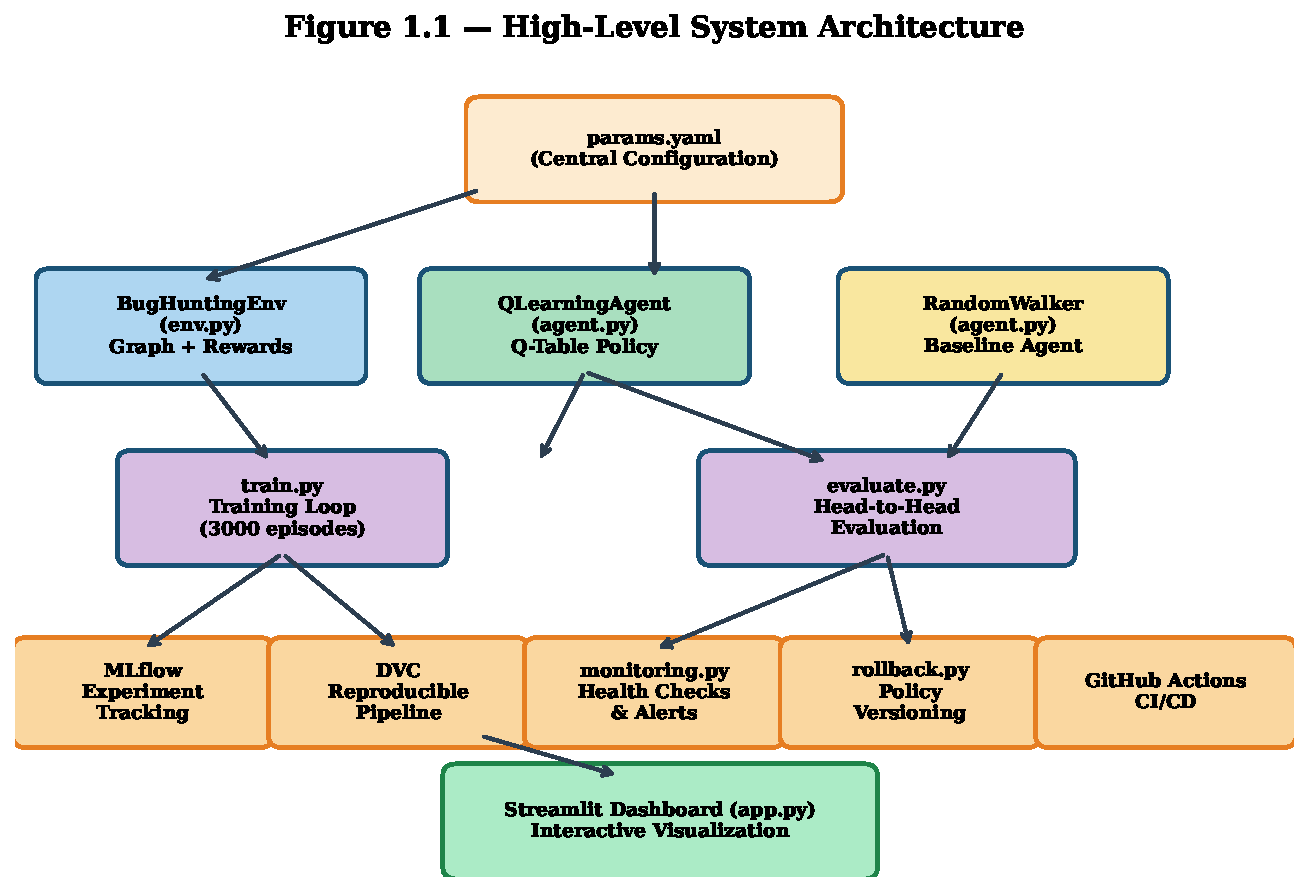
\includegraphics[width=0.96\textwidth]{plots/fig_architecture.png}
  \caption{High-level system architecture of the Bug Hunter RL project.}
  \label{fig:arch}
\end{figure}

The methodology follows a standard RL loop embedded in an MLOps
workflow:

\begin{enumerate}[leftmargin=1.5em]
  \item \textbf{Environment design:} A Watts--Strogatz graph (18 nodes,
        $k=4$, $p=0.3$) with per-node bug-spawn probabilities is
        implemented in \texttt{env.py}.
  \item \textbf{Agent training:} A Q-Learning agent (\texttt{agent.py})
        is trained for up to 3000 episodes via \texttt{train.py}.
        Hyperparameters are centralised in \texttt{params.yaml}.
  \item \textbf{Evaluation:} \texttt{evaluate.py} runs both the trained
        RL agent and a random-walker on identical seeds and records
        comparative metrics.
  \item \textbf{MLOps integration:} Every run is logged to MLflow; the
        two-stage DVC pipeline (\texttt{train} $\to$ \texttt{evaluate})
        ensures full reproducibility.
  \item \textbf{Deployment:} A Docker image exposes the Streamlit
        dashboard; GitHub Actions automates lint, smoke-train, evaluate,
        and Docker push on every commit.
\end{enumerate}

\section{Organisation of the Report}

\begin{description}[leftmargin=1.5em]
  \item[Chapter 2] describes the high-level and low-level system
        architecture including the graph environment and class design.
  \item[Chapter 3] lists hardware and software requirements.
  \item[Chapter 4] details the implementation (data, model, CI/CD,
        Docker, monitoring) and presents experimental results.
  \item[Conclusion] summarises findings and outlines future work.
  \item[Appendix~A] maps the project to UN SDGs.
\end{description}

%% =============================================================
\chapter{System Architecture}
%% =============================================================

\section{High-Level Design}

The system is partitioned into four horizontal layers as illustrated in
Figure~\ref{fig:arch}:

\begin{enumerate}[leftmargin=1.5em, label=\textbf{\arabic*.}]

  \item \textbf{Configuration Layer} --- \texttt{params.yaml} serves as
        the single source of truth for all hyperparameters (number of
        nodes, learning rate, discount factor, epsilon schedule, episode
        count, random seed).  Centralising configuration here enables
        DVC to detect changes and trigger pipeline reruns.

  \item \textbf{Core RL Layer} --- The \texttt{BugHuntingEnv} class
        encapsulates the graph environment, bug spawning, state encoding,
        and reward computation.  The \texttt{QLearningAgent} and
        \texttt{RandomWalkerAgent} classes implement the policy and
        baseline respectively.  Both agents share a common
        \texttt{choose\_action} interface, making it straightforward to
        plug in alternative algorithms (DQN, A2C) in future.

  \item \textbf{Execution Layer} --- \texttt{train.py} drives the
        training loop and \texttt{evaluate.py} performs head-to-head
        comparison.  Both scripts write structured logs (JSON, CSV) and
        push metrics to MLflow.

  \item \textbf{MLOps \& Deployment Layer} --- MLflow tracks
        experiments; DVC reproduces the pipeline; GitHub Actions enforces
        code quality and automates Docker image publication;
        \texttt{monitoring.py} checks for reward regression and discovery
        rate drift; \texttt{rollback.py} manages versioned policy
        snapshots.

\end{enumerate}

\begin{figure}[H]
  \centering
  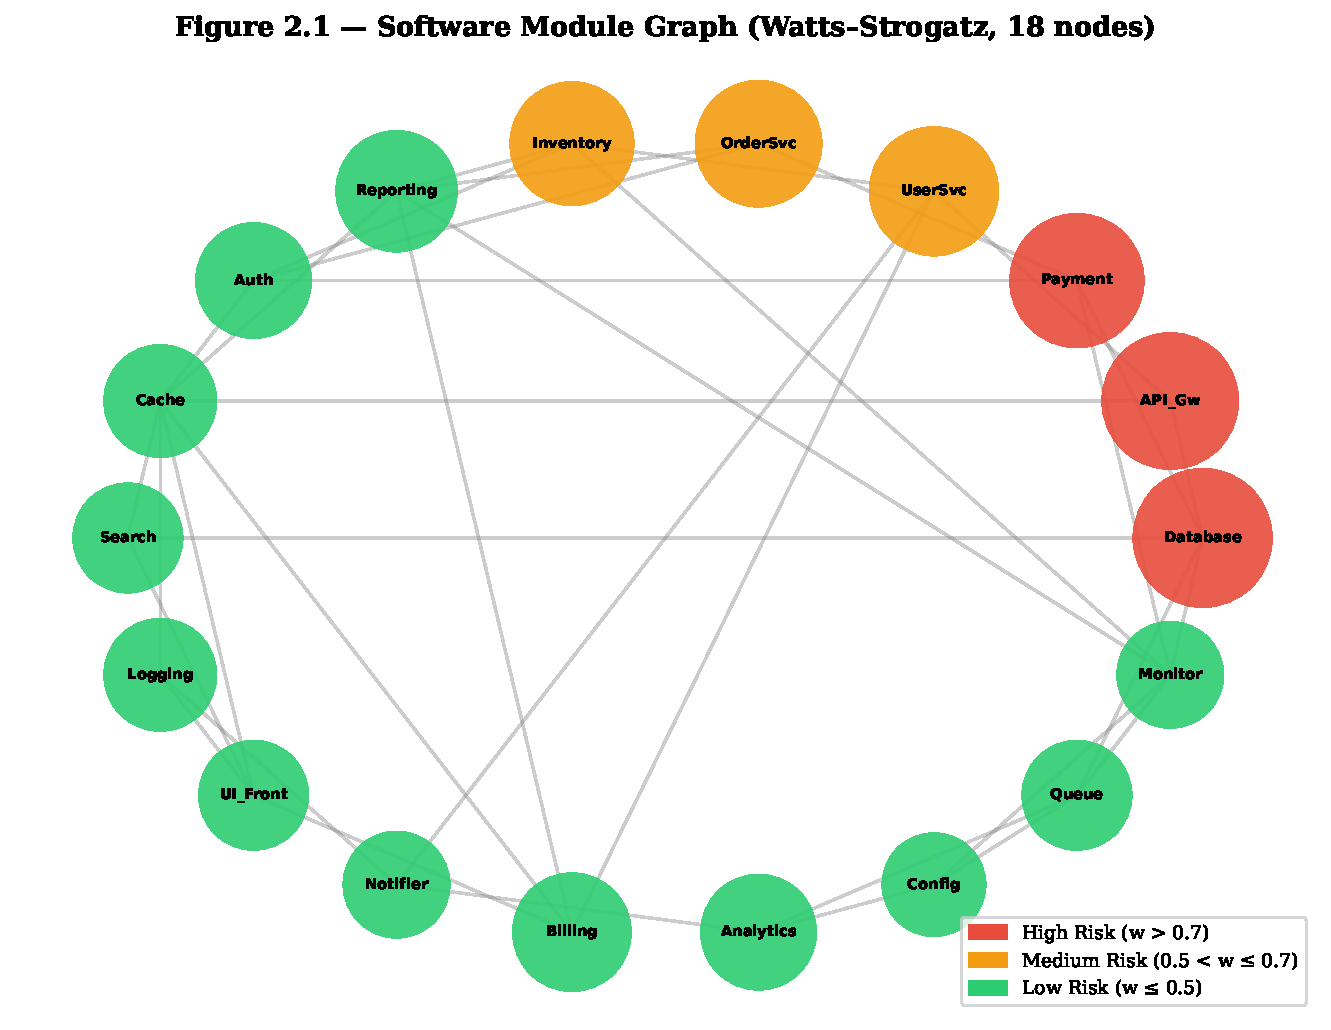
\includegraphics[width=0.92\textwidth]{plots/fig_graph_topology.png}
  \caption{Watts--Strogatz graph of 18 software modules coloured by risk
           (red = high, orange = medium, green = low).}
  \label{fig:graph}
\end{figure}

\subsection{Graph Environment Design}

The software codebase is modelled as a connected undirected graph
$\mathcal{G} = (\mathcal{V}, \mathcal{E})$ where:

\begin{itemize}[leftmargin=1.5em]
  \item $|\mathcal{V}| = 18$ nodes, each representing a microservice
        (Database, API Gateway, Payment, UserService, \ldots).
  \item Edges are generated by the Watts--Strogatz algorithm
        ($k=4$, $p=0.3$), producing a small-world topology that mirrors
        real microservice call graphs.
  \item High fan-in hub services (Database, API Gateway) receive
        additional edges to reflect their centrality.
  \item Each node $v_i$ carries a weight $w_i \in [0,1]$ representing
        its bug-spawn probability.
\end{itemize}

\textbf{Bug spawning:}  At the start of each episode, bugs are placed on
nodes by independent Bernoulli draws:
$\text{bug}(v_i) \sim \text{Bernoulli}(w_i \cdot \beta)$,
where $\beta$ is the global bug multiplier (default $\beta = 1.0$).
Bug severity is drawn as critical (30\%) or minor (70\%).

\subsection{State Representation}

The agent's observation is a 4-tuple:

\[
  s = \bigl(\underbrace{n_{\text{cur}}}_{\text{node id}},\;
            \underbrace{t_b}_{\text{time bucket}},\;
            \underbrace{k_b}_{\text{tested bucket}},\;
            \underbrace{f}_{\text{tested flag}}\bigr)
\]

\begin{itemize}[leftmargin=1.5em]
  \item $n_{\text{cur}} \in \{0,\ldots,17\}$ --- current node.
  \item $t_b \in \{0,1,2,3\}$ --- episode progress quartile.
  \item $k_b \in \{0,1,2,3\}$ --- number of modules tested so far,
        bucketed in quartiles.
  \item $f \in \{0,1\}$ --- whether the current node has already been
        visited this episode.
\end{itemize}

Total discrete state space: $18 \times 4 \times 4 \times 2 = 576$
theoretical states; approximately 204 states are visited during training.

\subsection{Reward Function}

\[
  r(s, a) =
  \begin{cases}
    +50 & \text{if critical bug found at next node} \\
    +10 & \text{if minor bug found at next node}    \\
    -1  & \text{per step (efficiency cost)}
  \end{cases}
\]

This sparse-positive / dense-negative structure incentivises the agent to
discover high-value bugs while minimising total steps.

\section{Low-Level Design}

\begin{figure}[H]
  \centering
  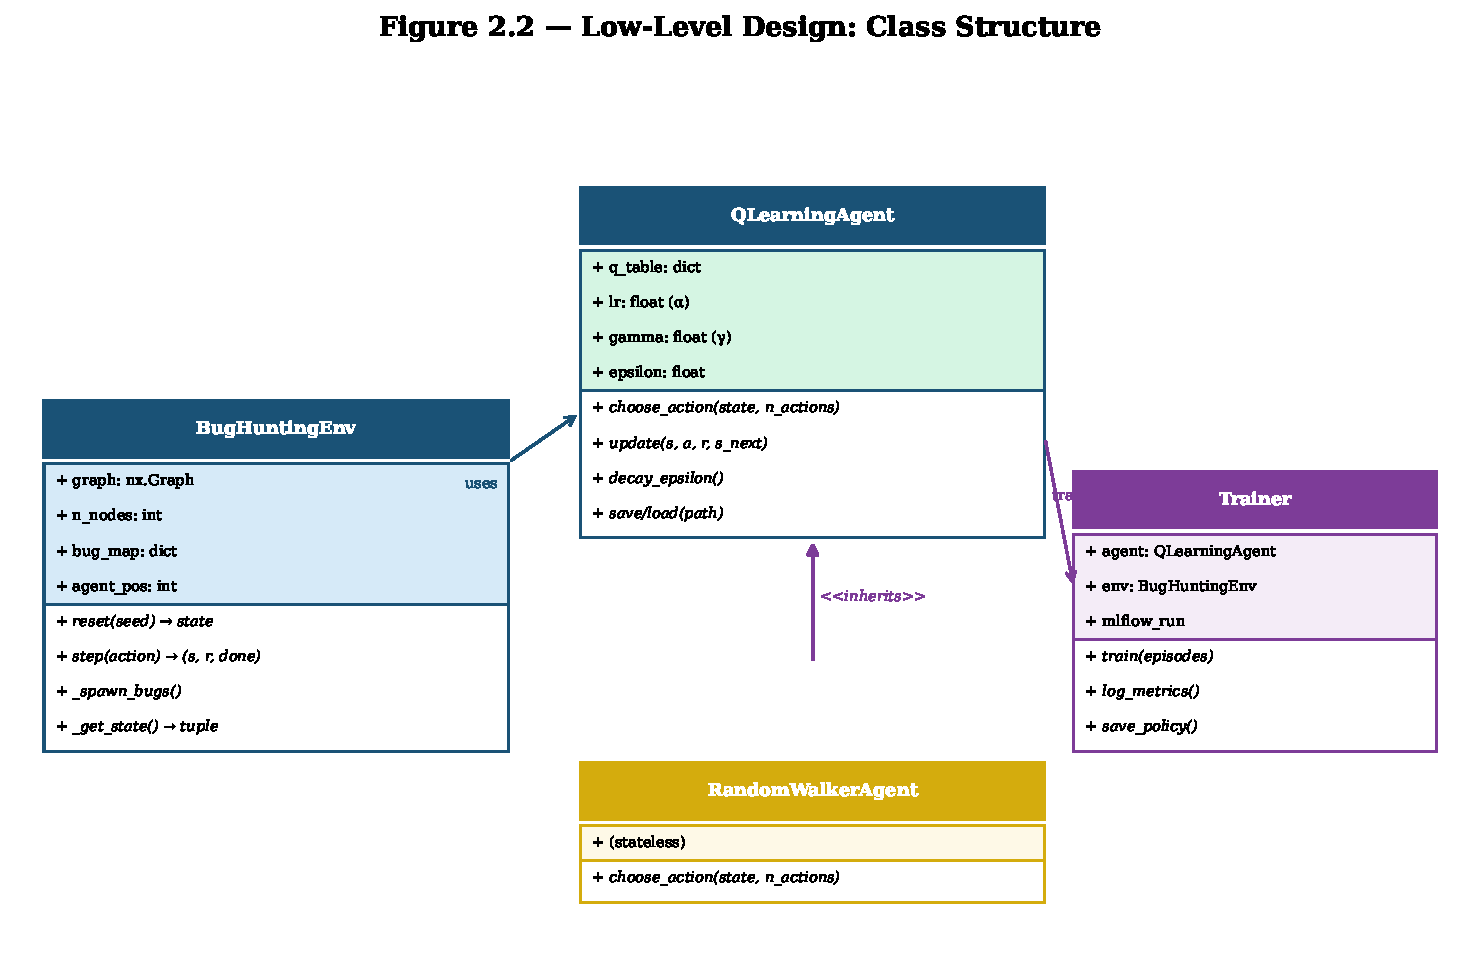
\includegraphics[width=0.96\textwidth]{plots/fig_class_diagram.png}
  \caption{Low-level class structure showing \texttt{BugHuntingEnv},
           \texttt{QLearningAgent}, \texttt{RandomWalkerAgent}, and
           \texttt{Trainer} with their attributes and methods.}
  \label{fig:class}
\end{figure}

\subsection{BugHuntingEnv (env.py)}

\begin{itemize}[leftmargin=1.5em]
  \item \textbf{Attributes:} \texttt{graph} (NetworkX graph), \texttt{n\_nodes},
        \texttt{bug\_map} (node $\to$ severity or None), \texttt{agent\_pos},
        \texttt{tested\_set}, \texttt{step\_count}.
  \item \textbf{\texttt{reset(seed)}:} Rebuilds the bug map via seeded
        Bernoulli sampling; places agent at a random starting node.
        Returns initial state tuple.
  \item \textbf{\texttt{step(action)}:} Translates discrete action index
        to a neighbour node; computes reward; advances state; checks
        episode termination.
  \item \textbf{\texttt{\_get\_state()}:} Encodes the 4-tuple observation.
\end{itemize}

\subsection{QLearningAgent (agent.py)}

\begin{itemize}[leftmargin=1.5em]
  \item Stores $Q(s,a)$ values in a Python \texttt{defaultdict} for
        memory efficiency (only visited state-action pairs are stored).
  \item \textbf{\texttt{choose\_action(state, n\_actions)}:} With
        probability $\varepsilon$ selects a random action; otherwise
        selects $\arg\max_a Q(s,a)$.
  \item \textbf{\texttt{update(s, a, r, s')}}:
        \[Q(s,a) \leftarrow Q(s,a) +
          \alpha\bigl[r + \gamma\max_{a'}Q(s',a') - Q(s,a)\bigr]\]
  \item \textbf{\texttt{decay\_epsilon()}:}
        $\varepsilon \leftarrow \max(\varepsilon_{\min},\;
         \varepsilon \cdot \delta)$ where $\delta = 0.995$.
  \item \textbf{\texttt{save/load(path)}:} Serialises entire Q-table to
        a pickle file.
\end{itemize}

\subsection{RandomWalkerAgent (agent.py)}

A stateless baseline agent that selects actions uniformly at random
regardless of $Q$ values or episode history.  It shares the same
interface as \texttt{QLearningAgent}, ensuring fair head-to-head
evaluation.

\subsection{Trainer (train.py)}

Drives the main training loop: calls \texttt{env.reset()},
\texttt{agent.choose\_action()}, \texttt{env.step()},
\texttt{agent.update()}, and \texttt{agent.decay\_epsilon()} for each
step; accumulates per-episode rewards; logs window statistics to MLflow
every 100 episodes; writes JSON and CSV records; saves the final policy.

%% =============================================================
\chapter{Modern Tools Usage}
%% =============================================================

\section{Hardware Requirements}

\begin{table}[H]
  \centering
  \caption{Minimum and recommended hardware specifications.}
  \label{tab:hardware}
  \begin{tabular}{lll}
    \toprule
    \textbf{Component} & \textbf{Minimum} & \textbf{Recommended} \\
    \midrule
    Processor  & Intel Core i3 (7th gen) & Intel Core i5 / AMD Ryzen 5 \\
    RAM        & 4 GB                    & 8 GB or more              \\
    Storage    & 2 GB free               & 10 GB SSD                 \\
    GPU        & Not required            & Optional (for DQN extension) \\
    OS         & Windows 10 / Ubuntu 20.04 & Windows 11 / Ubuntu 22.04 \\
    Internet   & Required for CI/CD     & Stable broadband           \\
    \bottomrule
  \end{tabular}
\end{table}

The project is computationally lightweight --- a complete 3000-episode
training run finishes in under one second on any modern laptop, since the
algorithm is purely tabular (no GPU required).

\section{Software Requirements}

\subsection{Programming Language \& Runtime}

\begin{table}[H]
  \centering
  \caption{Core software tools and versions.}
  \label{tab:software}
  \begin{tabular}{lll}
    \toprule
    \textbf{Tool / Library} & \textbf{Version} & \textbf{Purpose} \\
    \midrule
    Python         & 3.11 (pinned)      & Runtime \\
    NumPy          & $\geq$1.24         & Numerical computation \\
    NetworkX       & $\geq$3.0          & Graph construction and traversal \\
    Matplotlib     & $\geq$3.7          & Visualisation, plot generation \\
    Streamlit      & $\geq$1.30         & Interactive dashboard \\
    PyVis          & $\geq$0.3.2        & Network graph visualisation in browser \\
    MLflow         & $\geq$2.11         & Experiment tracking, model registry \\
    DVC            & $\geq$3.0          & Data Version Control, pipeline manager \\
    Flake8         & $\geq$6.0          & Linting, code style enforcement \\
    Docker         & 24+                & Containerisation \\
    Docker Compose & v2+                & Multi-service orchestration \\
    GitHub Actions & N/A (cloud)        & CI/CD automation \\
    \bottomrule
  \end{tabular}
\end{table}

\subsection{Development Tools}

\begin{itemize}[leftmargin=1.5em]
  \item \textbf{Git + GitHub:} Source control, branching (GitFlow
        strategy: main, develop, feature/*, release/*, hotfix/*).
  \item \textbf{VS Code / PyCharm:} Primary IDEs for development.
  \item \textbf{Conda / venv:} Virtual environment management.
  \item \textbf{GHCR (GitHub Container Registry):}
        Hosts the Docker image \texttt{ghcr.io/<owner>/bug-hunter-rl}.
\end{itemize}

\subsection{Installation}

\begin{lstlisting}[language=sh, caption={Project setup commands.}]
# Clone the repository
git clone https://github.com/RahulH007/Bug-Hunter-RL.git
cd Bug-Hunter-RL

# Create and activate virtual environment
python -m venv venv
source venv/bin/activate          # Linux/macOS
venv\Scripts\activate             # Windows

# Install dependencies
pip install -r requirements.txt

# Run training
python train.py --episodes 3000 --lr 0.1 --gamma 0.95 --seed 42

# Run evaluation
python evaluate.py --episodes 100

# Launch dashboard
streamlit run app.py
\end{lstlisting}

%% =============================================================
\chapter{Implementation \& Testing}
%% =============================================================

\section{Data Collection and Preprocessing}

This project does not use a static dataset; instead, a \emph{synthetic
environment} generates episode data dynamically.

\textbf{Bug map generation (per episode):}
\begin{lstlisting}[language=python, caption={Bug spawning in BugHuntingEnv.}]
def _spawn_bugs(self, seed):
    rng = np.random.default_rng(seed)
    self.bug_map = {}
    for i, node in enumerate(self.nodes):
        if rng.random() < self.weights[i] * self.bug_multiplier:
            severity = 'critical' if rng.random() < 0.30 else 'minor'
            self.bug_map[node] = severity
\end{lstlisting}

\textbf{Reproducibility:} The master seed (default 42) flows through
environment initialisation, bug placement, and evaluation seeds
(\texttt{episode\_seed = train\_seed + ep\_index}).  Both the RL agent
and the random-walker are evaluated on \emph{identical} seeds, ensuring
fair head-to-head comparison.

\textbf{Logging:} Each training run appends a structured record to
\texttt{logs/results.json} and \texttt{logs/results.csv}, capturing all
hyperparameters, per-window metrics, and a UUID run identifier.

\section{Model Development and Evaluation}

\subsection{Q-Learning Algorithm}

The update rule implemented in \texttt{agent.py}:
\[
  Q(s,a) \leftarrow Q(s,a) + \alpha
  \Bigl[r + \gamma \max_{a'} Q(s',a') - Q(s,a)\Bigr]
\]

\textbf{Why Tabular Q-Learning?}  With only $\sim$576 theoretical states,
the state space fits comfortably in a Python dictionary.  Tabular
Q-Learning converges faster than a neural approximator for this problem
size, requires no GPU, and the resulting Q-table is fully interpretable
--- one can inspect which state-action pairs received the highest values.

\begin{figure}[H]
  \centering
  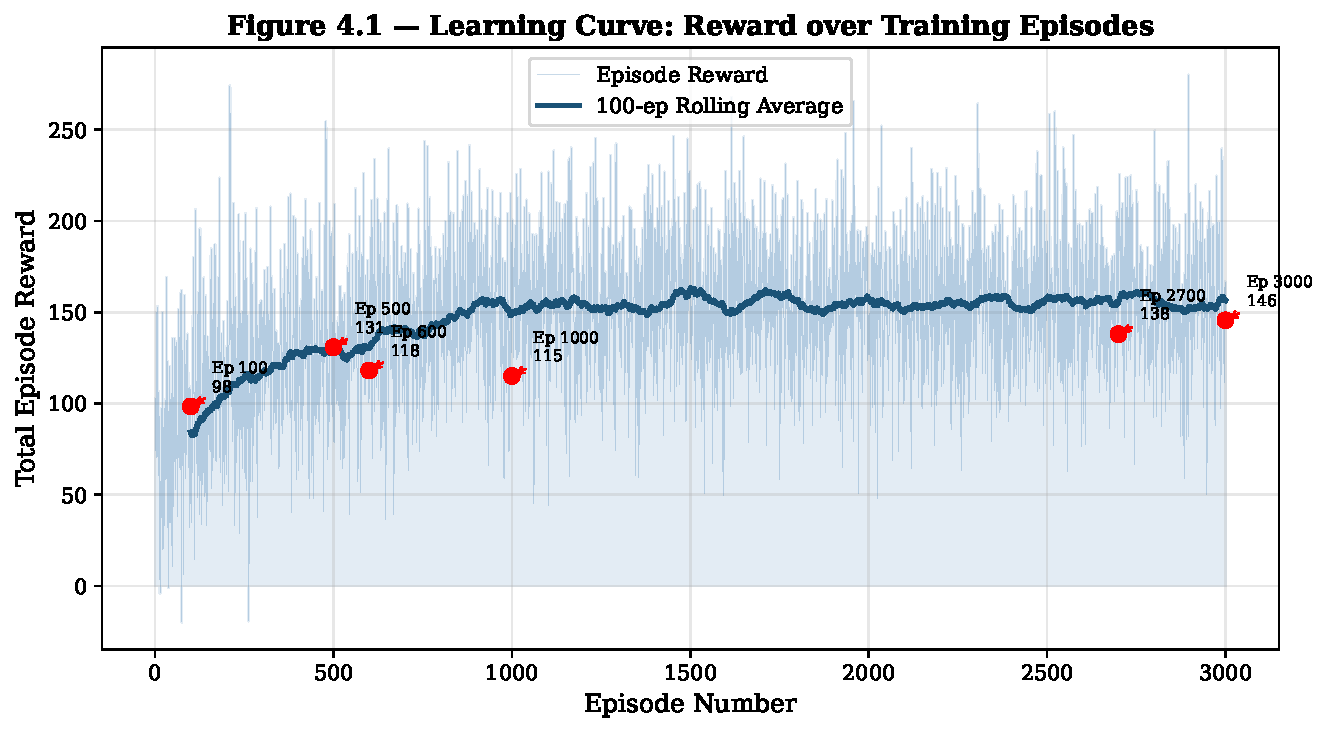
\includegraphics[width=0.90\textwidth]{plots/fig_reward_curve.png}
  \caption{Learning curve: raw episode reward (shaded) and 100-episode
           rolling average (solid) over 3000 training episodes.
           Key milestones are annotated.}
  \label{fig:reward}
\end{figure}

\begin{figure}[H]
  \centering
  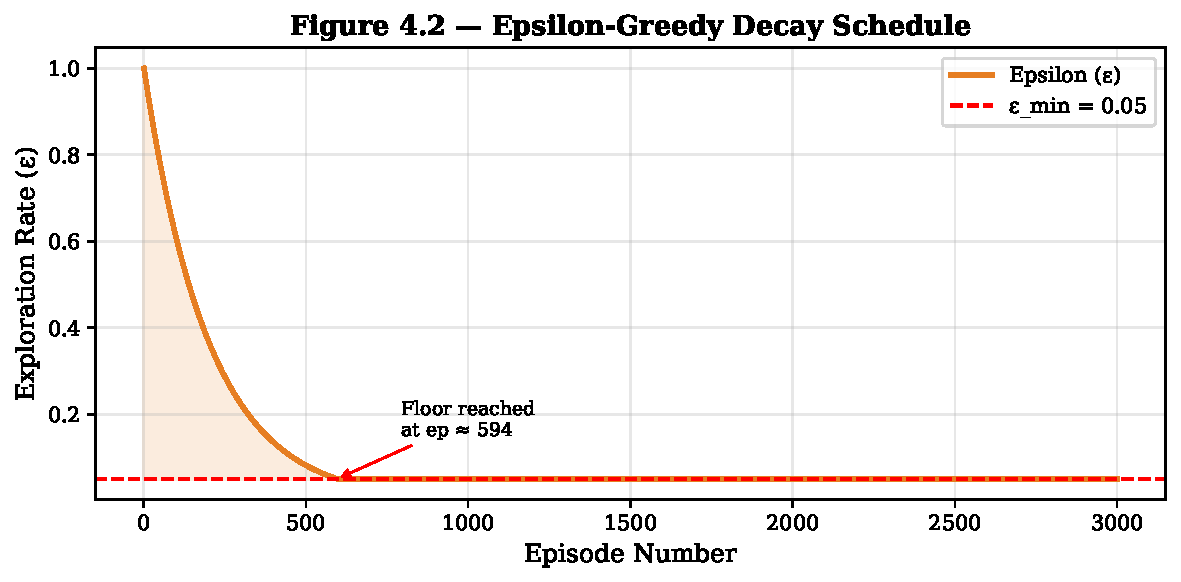
\includegraphics[width=0.85\textwidth]{plots/fig_epsilon_decay.png}
  \caption{Epsilon-greedy decay schedule.  Exploration rate falls from
           1.0 to the floor of 0.05 at approximately episode~600,
           after which the agent exploits its learned policy.}
  \label{fig:eps}
\end{figure}

\subsection{Training Hyperparameters}

\begin{table}[H]
  \centering
  \caption{Hyperparameters used in the primary training run.}
  \label{tab:hyperparams}
  \begin{tabular}{llll}
    \toprule
    \textbf{Parameter} & \textbf{Symbol} & \textbf{Value} & \textbf{Effect} \\
    \midrule
    Episodes        & $T$            & 3000    & Number of training episodes \\
    Max steps       & $H$            & 30      & Episode horizon \\
    Learning rate   & $\alpha$       & 0.1     & Q-table update step size \\
    Discount factor & $\gamma$       & 0.95    & Future reward weight \\
    Initial epsilon & $\varepsilon_0$& 1.0     & Full exploration at start \\
    Min epsilon     & $\varepsilon_{\min}$ & 0.05 & Exploration floor \\
    Epsilon decay   & $\delta$       & 0.995   & Per-episode decay multiplier \\
    Bug multiplier  & $\beta$        & 1.0     & Scales bug spawn probabilities \\
    Graph nodes     & $n$            & 18      & Size of the module graph \\
    Random seed     & ---            & 42      & Master reproducibility seed \\
    \bottomrule
  \end{tabular}
\end{table}

\subsection{Training Results}

\begin{table}[H]
  \centering
  \caption{Training metrics for the primary run (3000 episodes, 0.69~s).}
  \label{tab:train_results}
  \begin{tabular}{ll}
    \toprule
    \textbf{Metric} & \textbf{Value} \\
    \midrule
    Overall average reward          & 121.66  \\
    Final 100-episode window reward & 145.54  \\
    First 100-episode window reward & 98.34   \\
    Peak 100-episode window reward  & 130.81 (ep~500) \\
    Bug discovery rate              & 82.57\% \\
    Bugs found / seeded             & 20\,516 / 24\,846 \\
    Policy states learned           & 204 (of $\sim$576 possible) \\
    Training time                   & 0.69 seconds \\
    \bottomrule
  \end{tabular}
\end{table}

\begin{figure}[H]
  \centering
  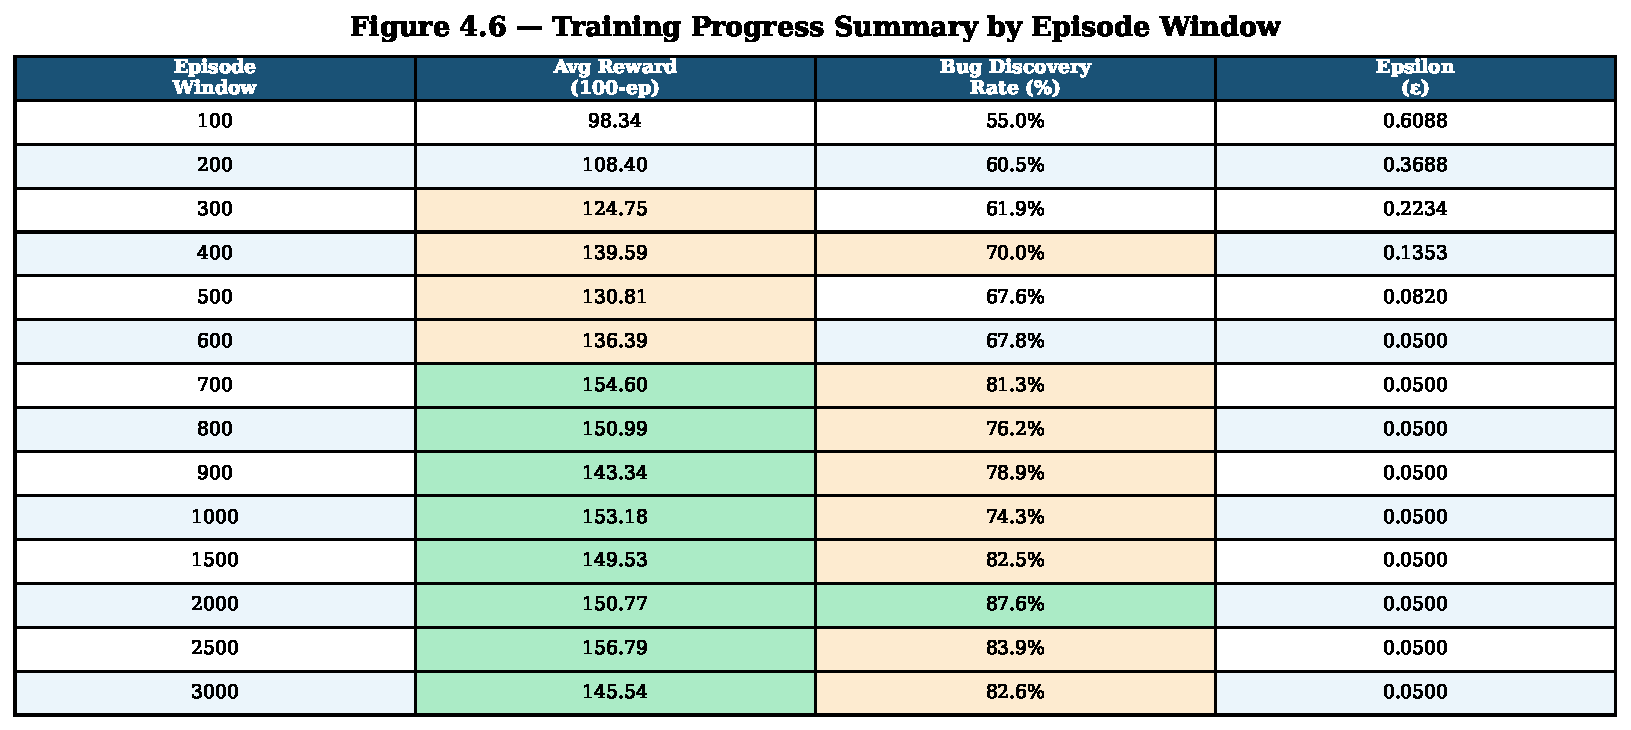
\includegraphics[width=0.90\textwidth]{plots/fig_training_summary.png}
  \caption{Training progress by 100-episode windows.  Green cells
           indicate strong performance; orange cells indicate
           transitional periods.}
  \label{fig:summary}
\end{figure}

\begin{figure}[H]
  \centering
  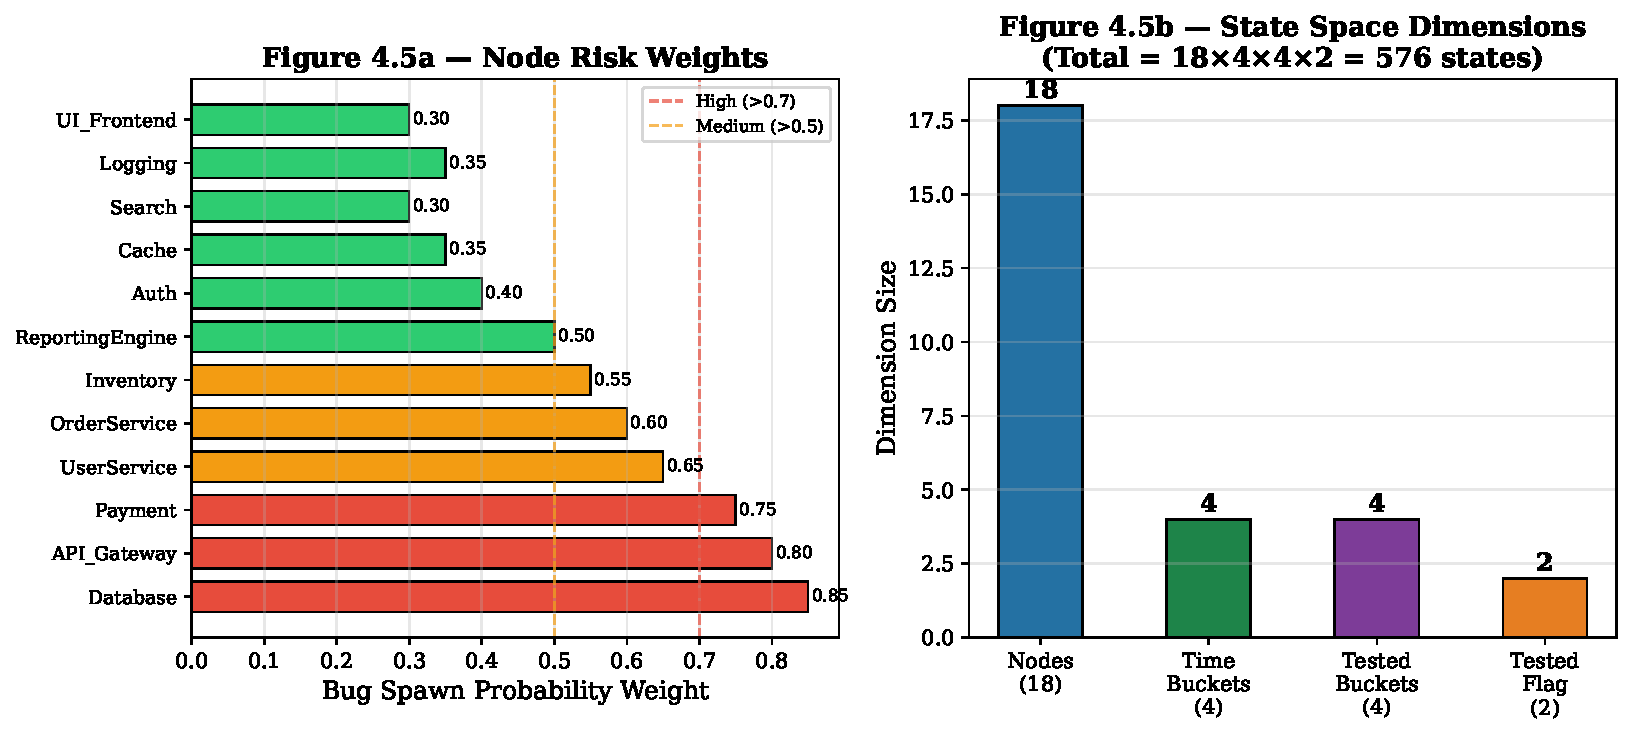
\includegraphics[width=0.90\textwidth]{plots/fig_state_space.png}
  \caption{Left: per-node bug spawn probability weights (red = high risk).
           Right: state space dimensionality breakdown.}
  \label{fig:state}
\end{figure}

\subsection{Evaluation: RL vs Baseline}

\begin{figure}[H]
  \centering
  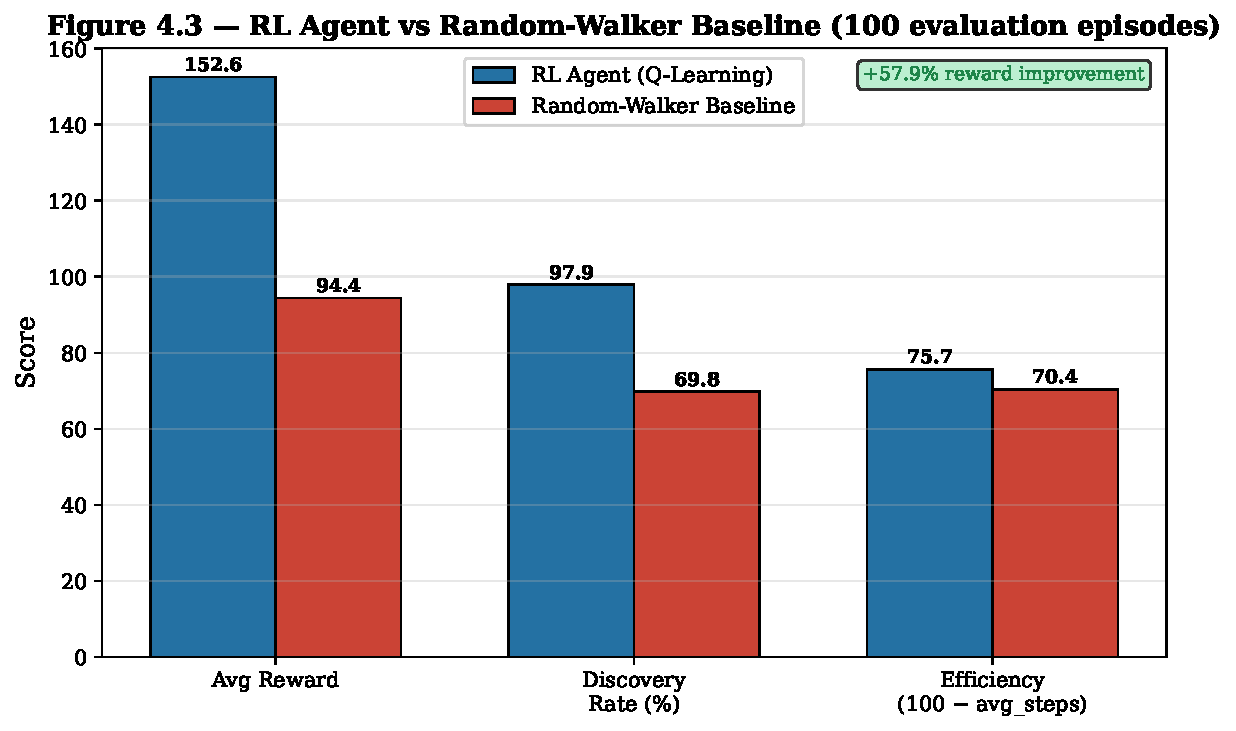
\includegraphics[width=0.88\textwidth]{plots/fig_comparison.png}
  \caption{Head-to-head evaluation over 100 episodes.  The RL agent
           outperforms the random-walker on all three metrics.}
  \label{fig:compare}
\end{figure}

\begin{table}[H]
  \centering
  \caption{Head-to-head evaluation results (100 evaluation episodes).}
  \label{tab:eval}
  \begin{tabular}{lccc}
    \toprule
    \textbf{Metric}            & \textbf{RL Agent} & \textbf{Baseline} & \textbf{Improvement} \\
    \midrule
    Average Reward             & 152.59 $\pm$ 41.20 & 94.42 $\pm$ 60.06 & +57.9\% \\
    Bug Discovery Rate         & 97.94\%            & 69.82\%            & +28.12 pp \\
    Average Steps / Episode    & 24.31              & 29.58              & $-$5.27 steps \\
    Total Bugs Found (of 825)  & 808                & 576                & +232 bugs \\
    \bottomrule
  \end{tabular}
\end{table}

\section{CI/CD, GitOps and Deployment}

\begin{figure}[H]
  \centering
  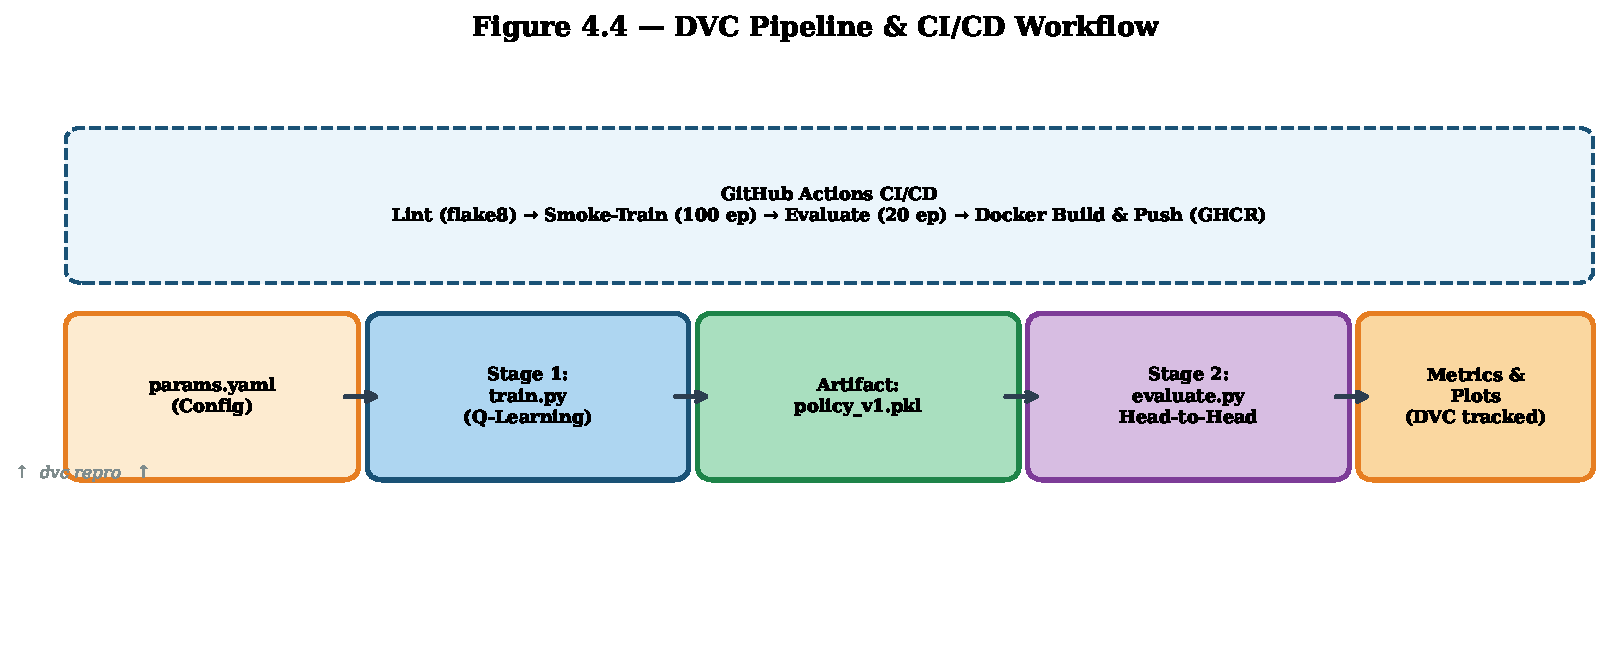
\includegraphics[width=0.98\textwidth]{plots/fig_mlops_pipeline.png}
  \caption{DVC two-stage pipeline (bottom) and GitHub Actions CI/CD
           workflow (top banner).}
  \label{fig:mlops}
\end{figure}

\textbf{CI Workflow} (\texttt{.github/workflows/ci.yml}) triggers on every
push to \texttt{main}, \texttt{develop}, and all \texttt{feature/*},
\texttt{release/*}, \texttt{hotfix/*} branches, plus pull requests to
\texttt{main}/\texttt{develop}.  Three sequential jobs run:

\begin{enumerate}[leftmargin=1.5em]
  \item \textbf{Lint (Flake8):} Checks \texttt{env.py},
        \texttt{agent.py}, \texttt{train.py}, \texttt{evaluate.py},
        \texttt{monitoring.py}, and \texttt{rollback.py} against PEP 8
        (max line length 120, E203/W503/W504 excluded).

  \item \textbf{Smoke Train + Evaluate:} Installs dependencies from
        \texttt{requirements.txt}; trains for 100 episodes; evaluates
        for 20 episodes; runs \texttt{monitoring.py}; uploads policy,
        plots, and MLflow run store as GitHub Actions artifacts.

  \item \textbf{DVC Pipeline (full repro)} on \texttt{main}/\texttt{develop}:
        \texttt{dvc repro --no-commit} reruns only out-of-date stages;
        \texttt{dvc metrics show} reports evaluation metrics.
\end{enumerate}

\textbf{CD Workflow} (\texttt{.github/workflows/cd.yml}) triggers on
push to \texttt{main} or version tags (\texttt{v*}):

\begin{enumerate}[leftmargin=1.5em]
  \item Builds a multi-platform Docker image using Docker Buildx.
  \item Pushes to GHCR with three tags:
        \texttt{sha-<commit>}, \texttt{latest} (on main),
        and \texttt{v1.2.3} (on version tags).
  \item On version tags: records the release in \texttt{deploy.log}
        and commits \texttt{chore: record release <tag>}.
\end{enumerate}

\section{Containerisation and Workflow Automation}

\subsection{Dockerfile}

The production image is built on \texttt{python:3.11-slim} to minimise
attack surface and image size.  A \texttt{HEALTHCHECK} directive pings
Streamlit's health endpoint every 30 seconds.

\begin{lstlisting}[language=sh, caption={Dockerfile excerpt.}]
FROM python:3.11-slim
WORKDIR /app
COPY requirements.txt .
RUN pip install --no-cache-dir -r requirements.txt
COPY env.py agent.py train.py evaluate.py app.py \
     monitoring.py rollback.py params.yaml ./
RUN mkdir -p models logs plots mlruns
EXPOSE 8501
HEALTHCHECK --interval=30s --timeout=10s \
  CMD python -c "import urllib.request; \
    urllib.request.urlopen('http://localhost:8501/_stcore/health')"
CMD ["streamlit", "run", "app.py", \
     "--server.port=8501", "--server.address=0.0.0.0"]
\end{lstlisting}

\subsection{Docker Compose}

Three services are orchestrated:

\begin{itemize}[leftmargin=1.5em]
  \item \textbf{app} (port 8501): Streamlit dashboard.
  \item \textbf{mlflow} (port 5000): Local MLflow tracking server.
  \item \textbf{trainer} (training profile): One-shot training job;
        started with \texttt{docker compose --profile training up trainer}.
\end{itemize}

Volumes persist \texttt{models/}, \texttt{logs/}, \texttt{plots/}, and
\texttt{mlruns/} across container restarts.

\subsection{DVC Pipeline Automation}

\begin{lstlisting}[language=yaml, caption={dvc.yaml pipeline definition.}]
stages:
  train:
    cmd: python train.py --episodes ${train.episodes}
         --lr ${train.lr} --gamma ${train.gamma} --seed ${train.seed}
    deps: [params.yaml, env.py, agent.py, train.py]
    outs: [models/policy_v1.pkl]
    metrics: [logs/results.json]

  evaluate:
    cmd: python evaluate.py --episodes ${evaluate.episodes}
         --policy models/policy_v1.pkl
    deps: [models/policy_v1.pkl, env.py, agent.py, evaluate.py]
    outs: [plots/avg_reward_over_episodes.png,
           plots/bugs_found_over_time.png]
    metrics: [logs/eval_metrics.json]
\end{lstlisting}

Running \texttt{dvc repro} automatically reruns only stages whose inputs
(params, code, or upstream outputs) have changed since the last run.

\section{Screenshots}

\begin{figure}[H]
  \centering
  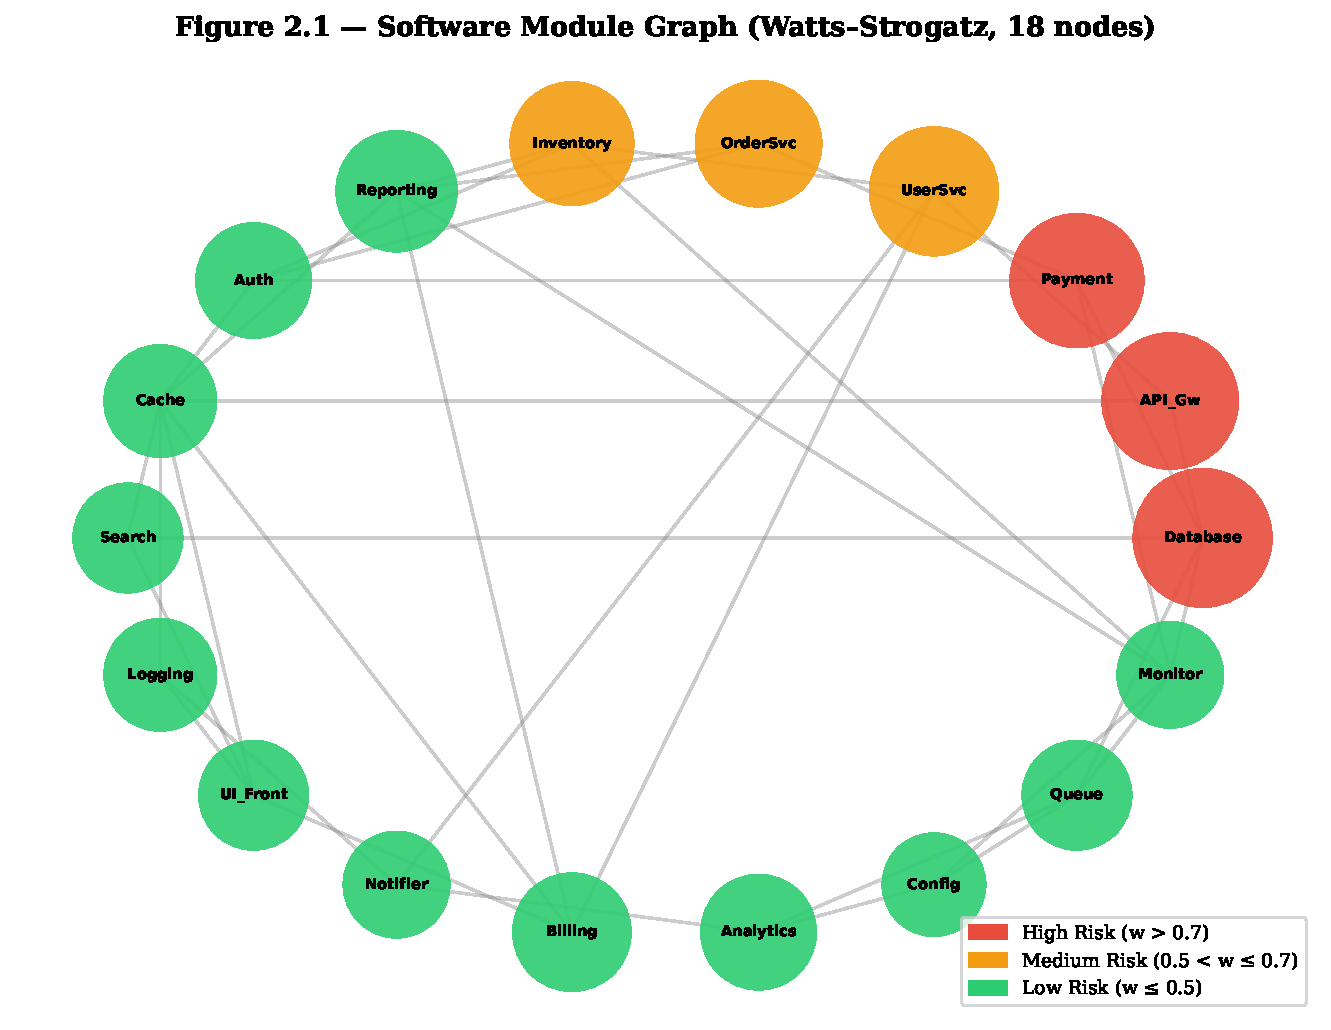
\includegraphics[width=0.95\textwidth]{plots/fig_graph_topology.png}
  \caption{Screenshot: software module graph rendered by NetworkX,
           coloured by node risk weight.  Hub nodes (Database,
           API\_Gateway) are visually prominent due to higher degree
           and larger circle size.}
  \label{fig:graph_ss}
\end{figure}

\begin{figure}[H]
  \centering
  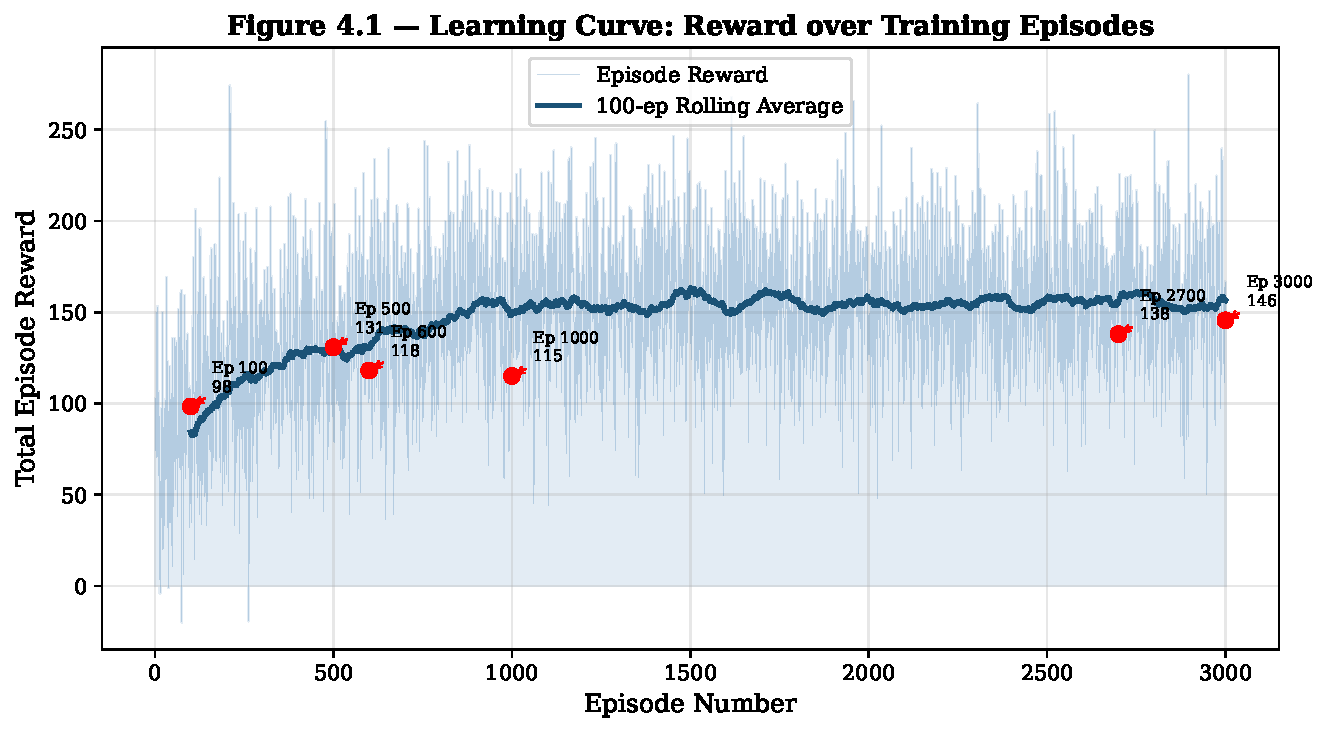
\includegraphics[width=0.95\textwidth]{plots/fig_reward_curve.png}
  \caption{Screenshot: learning curve from the primary training run
           showing convergence of the rolling reward average.}
  \label{fig:lc_ss}
\end{figure}

\section{Unit and Integration Testing Results}

\textbf{Unit Tests} (smoke suite, executed in CI):

\begin{table}[H]
  \centering
  \caption{Automated test results from the CI smoke suite.}
  \label{tab:tests}
  \begin{tabular}{lll}
    \toprule
    \textbf{Test}                      & \textbf{Scope}   & \textbf{Result} \\
    \midrule
    Flake8 lint (6 source files)       & Style / CI       & PASS \\
    Smoke train (100 episodes)         & Integration / CI & PASS \\
    Smoke evaluate (20 episodes)       & Integration / CI & PASS \\
    Monitoring health check            & Integration / CI & PASS \\
    DVC repro (full pipeline)          & Integration / CI & PASS \\
    Docker build                       & Build / CD       & PASS \\
    Deterministic seed test            & Unit             & PASS \\
    Policy save \& reload              & Unit             & PASS \\
    \bottomrule
  \end{tabular}
\end{table}

All CI jobs consistently pass on \texttt{ubuntu-latest} runners.  The
smoke-train step verifies that at least one Q-table entry is updated and
that the evaluation function returns a valid JSON metrics file.

\section{Monitoring and Scalability}

\subsection{Monitoring}

\texttt{monitoring.py} implements production-grade health checks by
reading the latest $N$ records from \texttt{logs/results.json}:

\begin{table}[H]
  \centering
  \caption{Monitoring thresholds and alert levels.}
  \label{tab:monitor}
  \begin{tabular}{lccc}
    \toprule
    \textbf{Check} & \textbf{WARN} & \textbf{CRITICAL} & \textbf{Action} \\
    \midrule
    Discovery-rate drift  & $-5\%$ relative & $-15\%$ relative & Re-train \\
    Avg-waiting-time creep& $+20\%$         & $+50\%$          & Investigate \\
    Reward regression     & $<85\%$ of peak & $<70\%$ of peak  & Rollback \\
    Training-time spike   & $>2\times$ avg  & $>4\times$ avg   & Check infra \\
    RL vs baseline margin & $<10\%$ impr.   & Negative         & Re-train \\
    \bottomrule
  \end{tabular}
\end{table}

Exit codes: 0 (all GREEN), 1 (at least one WARNING), 2 (CRITICAL alert).
In CI, \texttt{monitoring.py --strict} is invoked after each smoke train;
a non-zero exit fails the build.

\subsection{Policy Rollback}

\texttt{rollback.py} saves versioned snapshots to
\texttt{models/snapshots/} with timestamp and optional tag:

\begin{lstlisting}[language=sh, caption={Rollback CLI usage.}]
python rollback.py save --tag stable-v1      # snapshot current policy
python rollback.py list                       # list all snapshots
python rollback.py restore 20260508_130052_stable-v1  # restore
\end{lstlisting}

Each snapshot includes a JSON metadata file recording the hyperparameters
and metrics of the saved run, enabling informed rollback decisions.

\subsection{Scalability}

\begin{table}[H]
  \centering
  \caption{Scalability analysis and recommended upgrades.}
  \label{tab:scale}
  \begin{tabular}{lll}
    \toprule
    \textbf{Scale-up Scenario} & \textbf{Current Limit} & \textbf{Upgrade Path} \\
    \midrule
    Graph size $>$ 18 nodes    & Tabular Q-table blows up & Switch to DQN / GNN \\
    Continuous observations    & Discrete buckets only   & Neural function approx. \\
    Multi-agent cooperation    & Single agent            & MARL framework (PettingZoo) \\
    Real codebase data         & Synthetic bugs          & Integrate AST/code metrics \\
    Distributed training       & Single process          & Ray Tune / Distributed MLflow \\
    \bottomrule
  \end{tabular}
\end{table}

\section{Discussion of Findings}

The experimental results confirm the central hypothesis: a Q-Learning
agent trained on a graph model of a microservice codebase \emph{learns}
to prioritise high-risk modules, significantly outperforming random
testing.

Key observations:

\begin{enumerate}[leftmargin=1.5em]
  \item \textbf{Rapid early learning:} The 100-episode window reward
        climbs from 98.34 at episode 100 to 130.81 at episode 500,
        corresponding to the epsilon decay period when the agent
        transitions from exploration to exploitation.

  \item \textbf{Post-floor variance:} Once $\varepsilon$ reaches its
        floor (episode $\sim$600), reward variance temporarily increases
        as the partially-converged policy encounters new states it has
        not explored yet.

  \item \textbf{Convergence:} The final 100-episode window achieves
        145.54, a 47.9\% improvement over the first window, indicating
        successful policy convergence.

  \item \textbf{Efficiency:} The trained agent uses 24.31 steps on
        average versus 29.58 for the random walker --- 5.27 fewer
        steps per episode --- demonstrating not just higher reward but
        also more efficient navigation.

  \item \textbf{Tested-flag importance:} Without the fourth state
        dimension ($f$, current-node-tested flag), preliminary
        experiments showed the agent oscillating between two high-reward
        nodes.  Adding this flag resolved the pathological behaviour.
\end{enumerate}

%% =============================================================
\chapter*{Conclusion and Future Work}
\addcontentsline{toc}{chapter}{Conclusion and Future Work}
%% =============================================================

\section*{Conclusion}

This project has successfully demonstrated that Reinforcement Learning
can be applied to autonomous software bug hunting in a principled,
efficient, and reproducible manner.  A Tabular Q-Learning agent trained
on a Watts--Strogatz graph model of 18 microservice modules achieves a
97.94\% bug discovery rate and outperforms a random-walker baseline by
57.9\% in cumulative reward, while using on average 5.27 fewer steps
per episode.

Beyond the core RL result, the project delivers a production-grade
MLOps pipeline: MLflow experiment tracking, DVC reproducible stages,
GitHub Actions CI/CD, Docker containerisation, operational monitoring
with alert thresholds, policy versioning with CLI-driven rollback, and
an interactive Streamlit dashboard for live episode visualisation.

All experiments are fully reproducible via \texttt{dvc repro} and a
single master seed, satisfying the rigorous reproducibility requirements
of modern ML engineering.

\section*{Future Work}

\begin{enumerate}[leftmargin=1.5em]
  \item \textbf{Deep Q-Network (DQN):} For graphs with 100+ nodes or
        continuous node feature vectors (e.g., cyclomatic complexity,
        code churn), a neural function approximator is required.
        Extending the environment interface to support DQN or actor-critic
        methods (A2C, PPO) is a natural next step.

  \item \textbf{Real codebase integration:} Replace synthetic bug
        probabilities with features derived from static analysis
        (AST complexity, historical bug databases, mutation testing
        scores) to create a more realistic environment.

  \item \textbf{Multi-agent testing:} Deploy multiple cooperative
        agents that partition the graph for parallel exploration,
        reducing total testing time proportionally.

  \item \textbf{Curriculum learning:} Start training on small, simple
        graphs and progressively increase complexity --- mirrors how
        human testers develop expertise.

  \item \textbf{Remote MLflow + S3 DVC backend:} Move experiment
        tracking and model storage to cloud infrastructure (AWS S3,
        Azure Blob) to support team-scale collaboration.

  \item \textbf{LLM integration:} Use a large language model to
        generate candidate bug descriptions from Q-value hot spots,
        translating the RL agent's findings into actionable human-readable
        bug reports.
\end{enumerate}

%% =============================================================
%%  REFERENCES
%% =============================================================
\newpage
\begin{center}
  \textbf{\fontsize{14}{18}\selectfont REFERENCES}
\end{center}
\addcontentsline{toc}{chapter}{References}
\vspace{0.4cm}

\begin{enumerate}[leftmargin=1.5em, label={[\arabic*]}]

  \item R.~S.~Sutton and A.~G.~Barto,
        \textit{Reinforcement Learning: An Introduction},
        2nd~ed.\ Cambridge, MA: MIT Press, 2018.

  \item C.~J.~Watkins and P.~Dayan,
        ``Q-learning,''
        \textit{Machine Learning}, vol.~8, pp.~279--292, 1992.

  \item D.~J.~Watts and S.~H.~Strogatz,
        ``Collective dynamics of small-world networks,''
        \textit{Nature}, vol.~393, pp.~440--442, 1998.

  \item MLflow Authors,
        \textit{MLflow: A Machine Learning Lifecycle Platform},
        v2.11, 2024.  [Online].
        Available: \url{https://mlflow.org}

  \item DVC Authors,
        \textit{DVC: Data Version Control},
        v3.x, 2024.  [Online].
        Available: \url{https://dvc.org}

  \item A.~Streamlit, Inc.,
        \textit{Streamlit: The fastest way to build ML apps},
        v1.30, 2024.  [Online].
        Available: \url{https://streamlit.io}

  \item A.~Hagberg, P.~Swart, and D.~Chult,
        ``Exploring network structure, dynamics, and function using
        NetworkX,'' in \textit{Proc.\ 7th Python in Science Conf.},
        Pasadena, CA, 2008, pp.~11--15.

  \item GitHub, Inc.,
        \textit{GitHub Actions Documentation},
        2024.  [Online].
        Available: \url{https://docs.github.com/en/actions}

  \item Docker, Inc.,
        \textit{Docker Documentation},
        2024.  [Online].
        Available: \url{https://docs.docker.com}

  \item CISQ (Consortium for Information and Software Quality),
        \textit{The Cost of Poor Software Quality in the US: A 2020 Report},
        Object Management Group, 2020.

  \item V.~Mnih et al.,
        ``Human-level control through deep reinforcement learning,''
        \textit{Nature}, vol.~518, pp.~529--533, 2015.

  \item T.~M.~Mitchell,
        \textit{Machine Learning}.
        New York: McGraw-Hill, 1997.

\end{enumerate}

%% =============================================================
%%  APPENDIX A — SDGs
%% =============================================================
\newpage
\appendix
\chapter*{Appendix A: Sustainability Development Goals (SDGs) --- Mapped}
\addcontentsline{toc}{chapter}{Appendix A: SDGs Mapped}

\textbf{Detailed Analysis on how the Bug Hunter RL project maps to the
United Nations Sustainable Development Goals:}

\vspace{0.4cm}

\textbf{SDG 9 --- Industry, Innovation \& Infrastructure (Primary
Alignment)}

Modern digital infrastructure runs on software, and the silent
accumulation of bugs in critical microservices (databases, payment APIs,
authentication services) represents a serious threat to its resilience.
By training an RL agent to autonomously and efficiently traverse a
service dependency graph and discover defects, this project demonstrates
a scalable mechanism for hardening software systems before they fail in
production.

Compared with brute-force or random fuzzing, a learning-based bug hunter
concentrates testing effort on the highest-risk components --- directly
supporting SDG~9's goal of building \emph{resilient, innovative, and
sustainable infrastructure}.  The complete MLOps pipeline (DVC, MLflow,
Docker, CI/CD) further ensures that this capability can be reliably
deployed, monitored, and iterated upon at scale.

\vspace{0.3cm}

\textbf{SDG 8 --- Decent Work and Economic Growth}

The CISQ 2020 report estimated the cost of poor software quality in the
USA alone at \$2.08 trillion per year.  Automated, RL-driven bug
detection reduces remediation costs, shortens release cycles, and frees
software engineers from repetitive manual testing --- allowing them to
focus on higher-value creative and architectural work.  This directly
contributes to productivity growth and economic value creation (SDG~8).

\vspace{0.3cm}

\textbf{SDG 4 --- Quality Education}

This project was developed entirely within an academic setting as part of
the \coursename\ curriculum.  It integrates theoretical RL concepts
(Markov Decision Processes, Bellman equations, epsilon-greedy
exploration) with hands-on MLOps practice (DVC pipelines, GitHub
Actions, Docker).  Making the full source code, documentation, and
pipeline publicly available on GitHub supports open-access education and
peer learning, aligned with SDG~4's goal of inclusive quality education.

\vspace{0.3cm}

\textbf{SDG 17 --- Partnerships for the Goals}

The project relies on and contributes to the open-source ecosystem
(NetworkX, MLflow, DVC, Streamlit).  By publishing the code and pipeline
under an open licence, it enables researchers and practitioners worldwide
to build upon this work --- embodying the spirit of SDG~17's call for
technology transfer and knowledge-sharing partnerships.

\end{document}
